\chapter{Background}
\lhead{\emph{Background}}

In this chapter, background research is presented. This includes an overview of the current technologies in the area as well as the technologies used in this dissertation and a review of the current research.

\section{Test Automation}

One of the goals of automated testing is to reduce the number of manual test cases. It is important to note that automated testing does not completely remove the need for manual testing, instead it frees testers from repeating tedious tasks, and allows them to focus on exploratory analysis. Automated testing comes in many forms, such as Unit or Integration testing. There are also many agile methodologies around testing. So-called extreme programming allows for a number of practices around automated testing. For example, developers are encouraged to pair on many tasks. This involves both developers sitting in front of 2 screens which show the same code \cite{6901641}. It is important  with pairing not to sit in unnatural positions as pairing can take place over a number of hours, and developer health should be taken into consideration. During pairing, developers can write tests as they are developing software. One method called ping pong pairing involves one developer writing a failing unit test, the next developer will then make the failing test pass. Then the roles are reversed. This gives both developers a chance at writing both tests and implementations, increasing both of their understanding of the code base, while reducing siloed knowledge. 

One paradigm which is often used to describe what test automation is the testing pyramid which is depicted in figure \ref{fig:testing-pyramid}

\begin{figure}[!h]
  \centering
    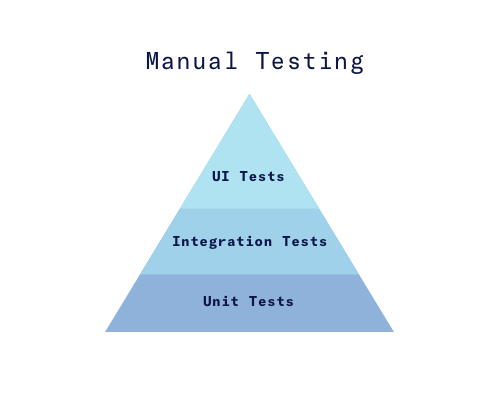
\includegraphics[width=0.8\textwidth]{figures/testing-pyramid.png}
    \caption{Testing pyramid}
    \label{fig:testing-pyramid}
\end{figure}

The testing pyramid states that tests on the bottom are fast running such as unit tests. They are relatively inexpensive to write. As we move up the pyramid we see that tests are much slower to run and become more expensive in terms of time to run and infrastructure required.

\section{Stress Testing}

Stress testing involves the process of simulating heavy traffic against an environment to see can that environment can handle the load. It is not clear where stress testing fits into the testing pyramid depicted in figure \ref{fig:testing-pyramid}. There are numerous stress testing tools on the market such as Apache JMeter \cite{jmeter}, WebLOAD \cite{webload} and LoadNinja \cite{loadninja}. These tools fit well into continuous integration environments. For example, when a developer pushes code changes to a code revision tool such as Git, continuous integration tools such as Jenkins can run a build which stress tests the changes using JMeter, if any of the code changes cause degradation then JMeter will detect this, possibly failing the build, meaning that the developer must fix the issue before they are allowed to merge their changes to a master branch. This prevents any performance degradations reaching production.

\section{Websockets}

Web sockets are a relatively new protocol, designed to enable real time communication between a client and a server. In the past there have been limited attempts at creating real-time communication. Some of these include polling and long polling of HTTP requests. With polling, a client will make multiple network requests to a server over a period of time. The server will respond with new data if it is available. This method has some limitations. It requires each request to initiate what is known as a handshake between the client and the server. Handshakes can take a number of milliseconds to initiate, while this is not apparent for a single network request, it becomes a problem when the server is dealing with many connections simultaneously \cite{5735801}. Handshakes traverse a number of stages as depicted in figure \ref{fig:http-handshake} before a successful connection is established. In the first stage a client will send a SYN packet. The server responds with a SYN-ACK, finally the client sends an ACK request and the connection is established \cite{5735801}. The complexity of this process is increased when the communication is encrypted using TLS (Transport Layer Security) as depicted in figure \ref{fig:https-handshake}. TLS is generally regarded as best practice, preventing hackers from snooping traffic on a network. This is made easy when TLS is absent, as all communication sent over a network is in plain text.

\begin{figure}[ht]
  \centering
    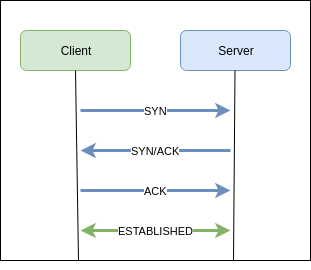
\includegraphics[width=0.5\textwidth]{figures/http-handshake.png}
    \caption{HTTP handshake}
    \label{fig:http-handshake}
\end{figure}

\begin{figure}[ht]
  \centering
    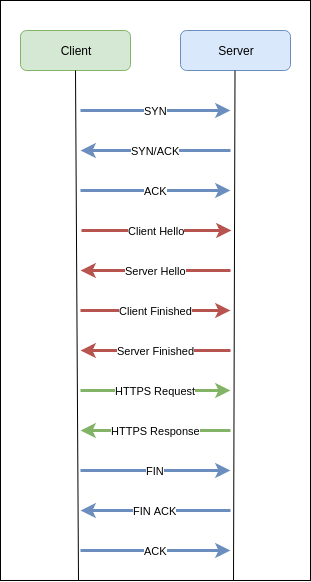
\includegraphics[width=0.5\textwidth]{figures/https-handshake.png}
    \caption{HTTP(s) handshake over TLS}
    \label{fig:https-handshake}
\end{figure}

Long polling is another method of near real time communication. With long polling the quantity of requests is less numerous when compared to polling, leading to less overhead when initiating handshakes. A client sends a request to a server, the server keeps the request open for a number of seconds. If the server has new data to send to the client it will terminate the request sending the data back in the response of the request. The client reconnects immediately and waits for more data to arrive. Long polling cannot perform bi-directional communication over one connection. To establish two way communication it needs two connections simultaneously \cite{6364271}. This gives long polling a clear disadvantage when compared to web sockets.

Issues with polling and long polling become substantial when dealing with mobile devices. Continuous connection cycles have a negative effect on the battery life of these devices \cite{6364271}. The explosion of mobile device usage in recent years \cite{6365155} has increased the importance of the need for a protocol that handles full real time connection over one connection.

Web sockets enable bi-directional communication between a client and a server over a single connection. Support for web sockets is available in all major browsers including mobile browsers \cite{websocket-browser-support}. Once a connection is established between client and server, both can communicate freely with the other in either direction. The connection that is initiated is persisted, meaning that it will only terminate when either the client or the server choose to disconnect. This can reduce the impact on a mobile devices battery.

The impact of web sockets on server resource usage can be substantial. A study which done a comparative analysis of polling versus web sockets found that polling increases the memory consumption over time compared to web sockets which maintained a fairly constant memory consumption throughout\cite{6601579}. In terms of bandwidth usage when comparing polling versus web sockets it was concluded that polling uses a larger amount of bandwidth over time, the reason for this was that polling required 256 bytes of extra data to be sent over the wire even if that 256 bytes of data is not used up, this means that in some cases there is can be a lot of white space sent over the network. The second reason was that the header data required for polling is significantly larger than that of a web sockets header\cite{6601579}.

Web socket servers can hold many hundreds of thousands of connections open simultaneously. Over time it is necessary to free memory and CPU resources to prevent the server from becoming overloaded. Web sockets support a keep-alive mechanism to tell the server that the client is still actively using the connection. This is done in the form of a PING/PONG request. The server will send a ping request to the client, if the client is still active then it will respond with a pong. If the client does not respond then the server is free to terminate the connection thereby freeing up resources. 

Microservice architectures compliment web sockets in a number of ways. In front of most microservice environments is an API gateway\cite{6885428}. This is a reverse proxy between a companies API layer and the end user. It acts as a security barrier preventing the user from having direct access to any of the underlying API's. Nginx is an example of a reverse proxy with web socket support. When a web socket connection is created Nginx will stream the web socket request onto the target service, the data will flow from the service through the gateway to the user's client. 

While microservices do well to compliment web sockets, there are cases where a microservice can be difficult for web sockets. Scaling applications is one such situation. Scaling means having multiple instances of the same service running at the same time with a load balancer in front which can choose the healthiest instance of a service to route requests to. Load balancing web sockets can be a complex operation depending on how a web socket server is set up. The issue occurs when a connection is established to a service, that connection is long lived if there is a drop in connection and the web socket server re-connects then it is possible that the new connection may be connected to a different instance of the server the web socket was previously connected to. For this reason, it is a good practice to make web socket servers stateless. Best practices suggest connecting the service to a backend queue such as RabbitMQ, Apache Kafka or Redis. This way if a connection unexpectedly terminates it has a lesser impact which instance the re-connection is routed to.

\section{Monitoring}

As mentioned briefly in Chapter 1 monitoring of microservices is a complex task. This is due to the distributed nature of microservices. Monitoring can take many forms, such as resource monitoring or usage monitoring and log monitoring. with resource monitoring, an attempt is made to try and track the amount of CPU and memory usage or number of disk input/output jobs over a period of time. This is a powerful metric if utilized effectively. Companies such as Netflix and Facebook, employ AB testing. which introduces new services that are meant to replace an existing service. For example, if there is a service that recommends shows to watch, which is a service Netflix provides. and developers need to rewrite this service in a new language, they can do this and then deploy the new service side by side with the existing service. The new service would accept the same inputs as the existing service however the outputs would only be persisted from the existing service. The developers can then monitor resources over a period of time, if they see that the new service has a lesser impact on resources than the existing service, this can be used as evidence to determine that the new service is a suitable replacement.

Usage monitoring, on the other hand, involves tracking the number of users that visit certain services. In the case of a web application, this can be the number of users that have visited a website. To get the most out of this, most monitoring tools allow the ability to break the visitor usage down into what routes they have visited. For example, if we have a route in our web application that is for listing friends of a user, we could track if this route is being used or not. This type of tracking is very valuable as it can be used to determine if the features of an application are providing value to a user. NewRelic \cite{new-relic} is a tool which provides this service as a cloud offering. With NewRelic, developers need to install an agent into their code. This agent will then communicate with the NewRelic service and store usage statistics. 

Log monitoring in microservices is difficult. As mentioned in Chapter 1 this is again due to the distributed nature of microservices. Developers are no longer dealing with one single log, they are instead dealing with a log from each connected service in the system. With larger environments, debugging systems can prove a laborious task. One common way that companies use to provide an easier debugging experience is alog aggregator. All logs from each of the services are forwarded to a central log service. One of the most common platforms for log aggregation is the ELK stack \cite{8311756}. which is short for Elasticsearch, Logstash, and Kibana. These are 3 individual open source tools, however, when combined they make a powerful log aggregation tool. ElasticSearch is a distributed search and analytics engine, it can be used to index any form of data for searching. Logstash is a lightweight data processing pipeline tool that can accept data from a number of sources and finally Kibana lets developers visualize search queries in elastic search and provides a powerful user interface. With the ELK stack in place, developers can search for keywords such as "ERROR" or "CRASH" that occurred in logs in a specific time frame, making debugging systems less monotonous. Logz.io \cite{logzio} is an example of a company who has taken this a step further. They have combined machine learning that can scan and make sense of each log input. Their system can actively inform developers of anything it finds in their logs that it has marked as interesting or potentially fatal. This reduces the workload of developers while debugging systems.

\section{Docker}

Docker is a tool that allows developers to create, deploy and run applications which are distributed as containers. Docker is often compared to virtualization tools such as Virtualbox and VMWare Fusion. We believe this comparison to be incorrect, the key difference being that virtualized run on top of a hypervisor which is running on top of a guest operating system, the running virtual machine has its own operating system such as Linux or Windows with its own memory management system. It is also possible to have multiple virtual machines running at the same time on a single machine. In comparison docker containers do not use a hypervisor, they are instead executed using the docker engine. Containers are considerably smaller and use fewer resources than virtual machines as well as having much faster startup times. Because of this docker containers are starting to be used for tasks such as integration testing.

Without docker, there was no real way to test an applications integration with a database such as MySql. When developers wrote tests they usually used an in-memory database such as H2. For example, if we are building a web application that has a rest endpoint for creating a shopping list we could write an integration test that would start the application and make a HTTP request to this endpoint and check if the endpoint stores our shopping list correctly. As the application is starting it would also start the in-memory H2 database. If the test passes we have some assurance that when our application reaches a production environment that it will just work. However, in reality, this is not always the case. In memory databases like H2 are not 100\% compatible with MySql, that being, some queries that work on H2 will not work on MySql and vice versa. Docker, on the other hand, allows developers to start a real MySql server within a Docker container for the duration of the integration test. Once the test completes the container is thrown away, ensuring that new tests will be using a completely fresh database. There are a number of libraries available that make starting and stopping of containers easy, such as \href{https://www.testcontainers.org/}{TestContainers} for Java and NodeJs.

\section{Kubernetes}

While docker can be useful for testing it is also a production-ready tool and works well in a microservice architecture. Docker Swarm and Kubernetes are the two main docker container orchestration tools on the market today. Docker Swarm was originally developed by docker themselves. This allows docker containers to be spread over a number of virtual or real machines, while docker swarm would handle all network activity between each of the containers by utilizing its own DNS server. Kubernetes was originally designed by Google, the project was originally called Borg while later changing to be called Kubernetes. Kubernetes was made open source by Google in 2014. It has many of the same features that docker swarm has including network and DNS. Kubernetes is also available as a cloud offering from GKE (Google Kubernetes Engine). 

Both Docker Swarm and Kubernetes allow defining microservices or infrastructure as code. For example, if we are building a microservices, we can define each of these microservices and the networking between them as code. This code can then be distributed to allow for repeatable environments. In the case of docker swarm, this code is defined in a file called docker-compose.yml. For Kubernetes there is a package manager called Helm which uses YAML files to orchestrate the environment.

\section{Cloud Foundry}

Cloud Foundry is a popular PaaS (Platform as a Service) system maintained by Pivotal Labs. One of its main goals is to make working with microservices easy for developers. Cloud Foundry uses a different container technology than we see in Kubernetes, instead of Docker it uses Droplets. Droplets allow users to specify run time environments known as buildpacks. For example, if we are building a NodeJS application we would use the NodeJS buildpack and if we were building a Java application we would use the Java buildpack. Droplets can then use the specified buildpack to provide a sandboxed environment to run an application. Resource limits can also be put on each running application, these include CPU, Memory, and Storage.

Cloud Foundry also supports the auto-scaling of applications. A developer can set thresholds on the amount of memory or CPU usage if this threshold is reached then the Cloud Foundry system will deploy another droplet alongside the existing droplets. In front of each droplet is a load balancer. The load balancer will route requests to each of the running instances of the applications in a round robin fashion.

Third party services such as MySql, Postgres, and MongoDB can be bound to applications. When binding services to an application the credentials of the service and connection URI will automatically be exposed to a running application in the form of environment variables. The application can then read these environment variables to connect to the service.

Cloud Foundry exposes a powerful rest API which can be used to query running applications and get usage statistics such as Memory CPU and storage of each running instance of an application. With this API it is also possible to get information on application states. As will be explained in Chapter 3 we will be utilizing this API to monitor running applications while we perform stress testing.

\section{Current State of the Art}

Automated testing has been utilized to great effect over the past 10 years due to the widespread adoption of agile methodologies. The journey from being a company not practicing agile to a company that does practice agile is a difficult one. Lawrence and YSlas suggested that cultural differences may play a part in this \cite{1667587}. Vriens and Barto suggested that senior management are often a roadblock in this transition, stating ``If this involvement by senior management results in micromanagement, the engineers will lose energy and self-direction resulting in an initiative-lacking organization`` \cite{4599511}. However, a successful transition will result in a highly collaborative and adaptive team free from the shackles of process.

Adopting a DevOps culture is key to being a successful agile practicing organization. One of the goals of DevOps is to bring software updates to production as quickly and as regularly as possible. To achieve this, organizations have to employ a high degree of automated testing. A study, conducted in 2019 concluded that performance evaluation of software was rarely used. The study found that only one-third of companies involved conducted performance evaluations on their systems. And 50\% of those who do performance evaluations spend only 5\% of their time working on these tests \cite{bezemer2019performance}. The study also presents a potential reason for this, stating that ``DevOps movement is
still in its infancy, and developers are still getting used to the opportunities that this movement offers in terms of automation of
performance engineering processes``.

Bezemer also suggests that the complexity involved in performance testing may act as a barrier for widespread adoption, and also concludes that current performance testing tools do not integrate well with current continuous integration tools such as Jenkins or TeamCity.

In our experience working in the software industry, these conclusions are accurate and from what we have seen, other forms of testing often take priority over performance testing. This can also be verified when looking at previous papers written on the subject. Weyuker states that often the primary issues that are reported from production environments are related performance degradation's when companies look into the reasons why this is the case, they usually find that there was no real test strategy for validating the performance of the application \cite{888628}. 